\section{Multi-Purpose Detectors}
\paragraph{a)}
\begin{figure}[H]
	\centering
	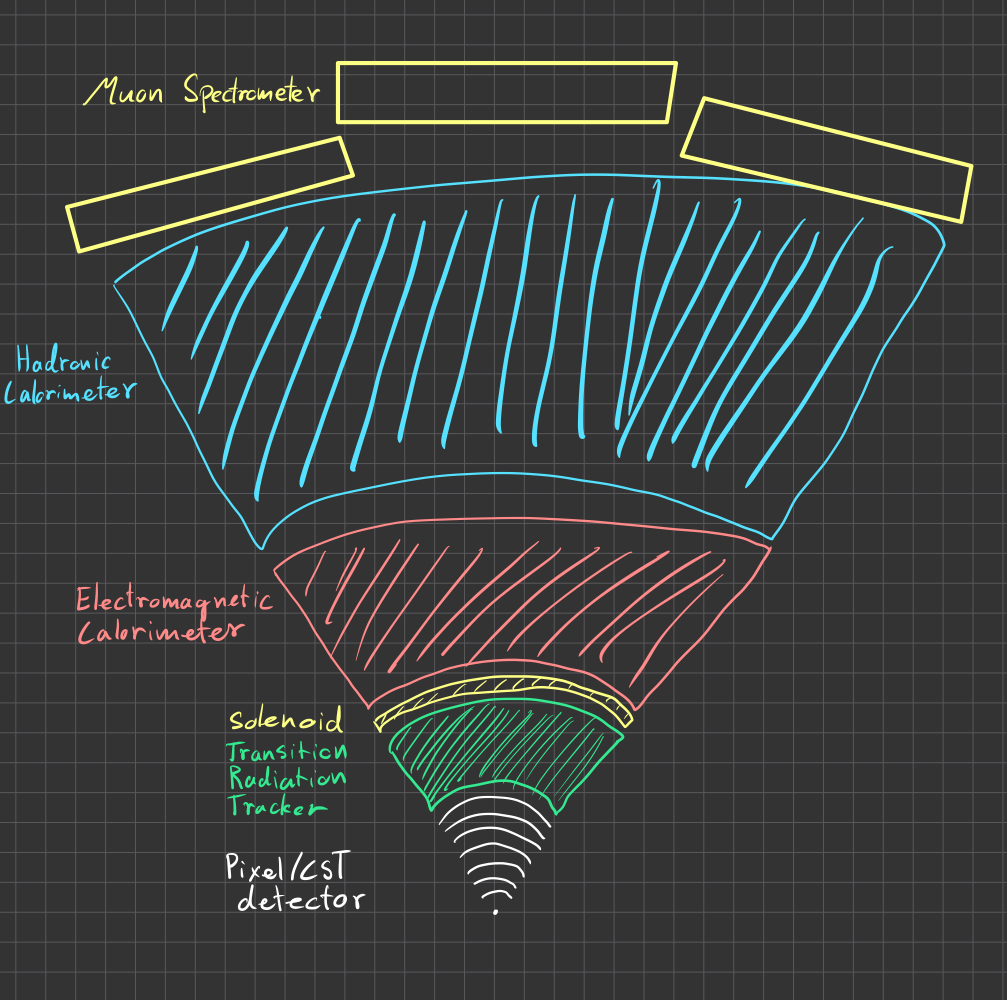
\includegraphics[width=\textwidth]{figures/Atlas.jpeg}
	\caption[]{The `onion' layout of a generic multi-purpose detector.}
\end{figure}

\paragraph{b)} The Pixel/CST tracker and the Transition radiation tracker measures the direction, momentum, and charge of electrically charged particles which are produced in the collisions of hadrons inside the accelerator. The solenoid bends charged particle to measure the momentum of them. The electromagnetic calorimeter measures the energy of particles which are interacting electromagnetically. The hadronic calorimeter measures the energy of hadrons. The muon spectrometer are used to detect muons and measure the muon's properties.

\paragraph{c)} Photons doesn't show upp in the tracker since they are not charged, but showers in the electromagnetic calorimeter. Muons go almost straight through the detector showing up in all section, bending a little and being are also measured by the muon spectrometer. Charged hadrons bends from the solenoid, shows up in the tracker, and shows up, but goes through the electromagnetic calorimeter and then showers in the hadronic calorimeter. Neutral hadrons go straight to the hadronic calorimeter and showers there.

\paragraph{d)} The candidate $p p \to \text{2 jets}$ is most likely Figure 2 and 4. Since there are two large showers in the hadronic calorimeter and they are 180 degrees apart.

The candidate $Z \to \mu \mu$ is most likely Figure 1. There are two directions where muons are detected in the muon spectrometer. Thus we should have a reaction with 2 muon products.

The candidate $J/\Psi \to e e$ is most likely Figure 3. There are two showers in the electromagnetic calorimeter, which matches the reactions with two electrons.

The candidate $W \to \mu \nu_\mu$ has no figure with a good match. We would want a detection in muon spectrometer along one line, and nothing more.

